\section{SDEs for arbitrary width}

\label{2305:app:SDE_with_generic_width}
In this appendix we generalize the discussion of the spherical constrained SDE to network of arbitrary width.
As we already did at beginning of Section~\ref{2305:sec:width}, we fix the second layer to \(a_j=1\) for everything that follows.
\subsection{Unconstrained SDE with $p>1$}
The updates of overlapping matrix elements can be written as
\[\begin{split}
  \dif \Q_{jl} &= \frac{-\gamma (\w_j\cdot\nabla_{\w_l}{\ell}+\w_l\cdot\nabla_{\w_j}{\ell}) + \gamma^2\nabla_{\w_j}{\loss}\cdot\nabla_{\w_l}{\loss}}{d} = \frac{\gamma}{pd} \mathcal{Q}_{jl}, \\
  \dif m_{j} &= \frac{-\gamma \w_\star\cdot\nabla_{\w_j}\ell}{d}  = \frac{\gamma}{pd} \mathcal{M}_{j}.
\end{split}\]
where we recalled the definition of the random variables \(\mathcal{M}_{j}\) and \(\mathcal{Q}_{jl}\); the factor \(\sfrac1p\) is missing, but it will come out from the gradients \(\nabla_{\w_j}\).
As we already seen, the usual argument provides setting \(\dif t = \sfrac{\gamma}{pd}\) and say that the remaining factor is concentrating to its expected value
\[\begin{split}
    \dif m_{j} &= \Psi_{j} \dif t \\
    \dif \Q_{jl} &= \Phi_{jl} \dif t,
\end{split}\]
where \(\Phi_{jl} = \EV{\mathcal{Q}_{jl}}\) and \(\Psi_{j} = \EV{\mathcal{M}_{j}}\).
We can now go beyond this and add corrections to concentration, namely adding a Brownian motion, following \cite{arous2022high}:
\begin{equation}\label{2305:eq:SDE_p_generic}\begin{split}
    \dif \M_{j} &= \Psi_{j} \dif t + \sqrt{\frac{\gamma}{pd}}\vec{\sigma}^\M_{j}\cdot \dif \vec{B}_t \\
    \dif \Q_{jl} &= \Phi_{jl} \dif t + \sqrt{\frac{\gamma}{pd}}\vec{\sigma}^\Q_{jl}\cdot \dif \vec{B}_t.
\end{split}\end{equation}
The \(\vec{\sigma}^\M_{j}\) and \(\vec{\sigma}^\Q_{jl}\) are the rows of the matrix obtained by taking the square root of the covariance matrix of all the \(p+p^2\) random variable \(\mathcal{M}_{j}\) and \(\mathcal{Q}_{jl}\):
\begin{equation}\label{2305:eq:generic_p_variance}
  \begin{pmatrix}
    \vec{\sigma}^\M_{1}\\
    \vdots\\
    \vec{\sigma}^\M_{p}\\
    \vec{\sigma}^\Q_{11}\\
    %\vec{\sigma}^\Q_{12}\\
    % \vdots \\
    % \vec{\sigma}^\Q_{1p}\\
    % \vec{\sigma}^\Q_{22}\\
    \vdots \\
    % \vec{\sigma}^\Q_{2p}\\
    % \vdots\\
    \vec{\sigma}^\Q_{pp}
  \end{pmatrix}
  \coloneqq
  \scalebox{0.85}{$\sqrt{
    \begin{pmatrix}
        \Var{\left[\mathcal{M}_1\right]} &
        \cdots &
        \Cov{\left[\mathcal{M}_1,\mathcal{M}_{p}\right]} &
        \Cov{\left[\mathcal{M}_1,\mathcal{Q}_{11}\right]} &
        % \cdots &
        % \Cov{\left[\mathcal{M}_1,\mathcal{Q}_{1p}\right]} &
        % \Cov{\left[\mathcal{M}_1,\mathcal{Q}_{22}\right]} &
        \cdots &
        \Cov{\left[\mathcal{M}_1,\mathcal{Q}_{pp}\right]} \\
        %
        \vdots & \ddots & \vdots & \vdots & \ddots & \vdots \\
        %
        \Cov{\left[\mathcal{M}_p,\mathcal{M}_{1}\right]} &
        \cdots &
        \Var{\left[\mathcal{M}_p\right]} &
        \Cov{\left[\mathcal{M}_p,\mathcal{Q}_{11}\right]} &
        \cdots &
        \Cov{\left[\mathcal{M}_p,\mathcal{Q}_{pp}\right]} \\
        %
        \Cov{\left[\mathcal{Q}_{11},\mathcal{M}_{1}\right]} &
        \cdots &
        \Cov{\left[\mathcal{Q}_{11},\mathcal{M}_{p}\right]} &
        \Var{\left[\mathcal{Q}_{11}\right]} &
        \cdots &
        \Cov{\left[\mathcal{Q}_{11},\mathcal{Q}_{pp}\right]} \\
        %
        \vdots & \ddots & \vdots & \vdots & \ddots & \vdots \\
        %
        \Cov{\left[\mathcal{Q}_{pp},\mathcal{M}_{1}\right]} &
        \cdots &
        \Cov{\left[\mathcal{Q}_{pp},\mathcal{M}_{p}\right]} &
        \Cov{\left[\mathcal{Q}_{pp},\mathcal{Q}_{11}\right]} &
        \cdots &
        \Var{\left[\mathcal{Q}_{pp}\right]}
    \end{pmatrix}
  }$},
\end{equation}
and  \(\dif \b_t\) is a \(p(1+p)\)-dimensional Wiener process.

\subsection{Spherical Constrained SDE}
Let's move now to the actual spherical derivation. The steps used are exactly the same we did in \ref{2305:app:spherical_constraint},  Since we are forcing the weight on the sphere, the update rule that has to be used is
\[
  \w_j^{\i+1} =\frac{\w^\i_j - \gamma \nabla_{\w_j}{\loss}}{\left\|\w^\nu_j - \gamma \nabla_{\w_j}{\loss}\right\|}\sqrt{d};
\]
We introduce now \(\mathfrak{M}_{j}\) and \(\mathfrak{Q}_{jl}\) to discriminate between the spherical variable and the unconstrained ones. Multiplying both sides of the update rule by \(\w_\star\) and subtracting \(\mathfrak{M}_{j}\) we get
\[
  \dif \mathfrak{M}_{j} = \frac{\mathfrak{M}_{j} +\dif m_{jr}}{\left\|\w_j - \gamma \nabla_{\w_j}{\loss}\right\|}\sqrt{d} - \mathfrak{M}_{j}.
\]
Similarly, the product of two update rules brings us to
\[\begin{split}
    \dif\mathfrak{Q}_{jl} &= \frac{\w_j - \gamma \nabla_{\w_j}{\loss}}{\left\|\w_j - \gamma \nabla_{\w_j}{\loss}\right\|} \frac{\w_l - \gamma \nabla_{\w_l}{\loss}}{\left\|\w_l - \gamma \nabla_{\w_l}{\loss}\right\|} - \mathfrak{Q}_{jl} \\
        &= \frac{\mathfrak{Q}_{jl}+\dif \Q_{jl}}{\left\|\w_j - \gamma \nabla_{\w_j}{\loss}\right\|\left\|\w_l - \gamma \nabla_{\w_l}{\loss}\right\|}d- \mathfrak{Q}_{jl}
\end{split}\]
Let's estimate the normalization factor
\[
  \begin{split}
  \left\|\w_{j} - \gamma \nabla_{\w_j}{\loss}\right\| =& \sqrt{(\w_{j} - \gamma \nabla_{\w_j}{\loss})^2}
                                            =  \sqrt{\w_{j}^2 - 2\w_{j}\cdot\gamma \nabla_{\w_j}{\loss}+\gamma^2\left\|\nabla_{\w_j}{\loss}\right\|^2} \\
                                            =& \sqrt{d}\sqrt{\frac{\w_{j}^2}{d} + \frac{- 2\w_{j}\cdot\gamma \nabla_{\w_j}{\loss}+\gamma^2\left\|\nabla_{\w_j}{\loss}\right\|^2}{d}}
                                            = \sqrt{d}\sqrt{\Q_{jj} +\dif \Q_{jj}} \\
                                            =& \sqrt{d}\sqrt{1 +\dif \Q_{jj}},
  \end{split}
\]
Expanding up to leading orders we get
\[\begin{split}
  \dif \mathfrak{M}_{j} =& (\mathfrak{M}_{j} +\dif m_{jr})(1 +\dif \Q_{jj})^{-\frac12} - \mathfrak{M}_{j} \\
            =& (\mathfrak{M}_{j} +\dif m_{jr})\left(1 -\frac12\dif \Q_{jj} + \frac38\dif q^2_{jj}\right)-\mathfrak{M}_{j} \\
            =& \dif m_{jr} - \frac{\mathfrak{M}_{j}}{2}\dif \Q_{jj} -\frac12 \dif m_{jr} \dif \Q_{jj} + \frac38 \mathfrak{M}_{j} \dif \Q_{jj}^2
\end{split}\]
\[\begin{split}
  \dif\mathfrak{Q}_{jl} =& (\mathfrak{Q}_{jl} +\dif \Q_{jl})(1 +\dif \Q_{jj})^{-\frac12}(1 +\dif \Q_{ll})^{-\frac12} - \mathfrak{Q}_{jl} \\
            =& (\mathfrak{Q}_{jl} +\dif \Q_{jl})\left(1 -\frac12\dif \Q_{jj} + \frac38\dif q^2_{jj}\right)\left(1 -\frac12\dif \Q_{ll} + \frac38\dif q^2_{ll}\right)-\mathfrak{Q}_{jl} \\
            =& \dif \Q_{jl} - \frac{\mathfrak{Q}_{jl}}{2}(\dif \Q_{jj}+\dif \Q_{ll}) + \frac{\mathfrak{Q}_{jl}}{8}(3\dif \Q_{jj}^2+3\dif \Q_{ll}^2 + 2\dif \Q_{jj}\dif \Q_{ll})-\frac12(\dif \Q_{jl}\dif \Q_{jj}+\dif \Q_{jl}\dif \Q_{ll})
\end{split}\]

We can now use the Itô Lemma on differentials Equations~\eqref{2305:eq:SDE_p_generic},
obtaining 
\[
  \dif x_a \dif x_b = \frac{\gamma}{pd}\vec{\sigma}_{x_a} \cdot \vec{\sigma}_{x_b}\dif t, \quad
\]
so we have some extra drift terms at an higher order.

\subsection{Special cases}
Computing explicitly the variance in Equation~\eqref{2305:eq:generic_p_variance} is not conceptually different from what exposed in Appendix~\ref{2305:app:square_equations}: expanding all the expression we are left expectations of polynomials of the preactivations.
Even if not complex, it is required to compute up to twelfth moments of a multivariate normal distributions, that could lead to very long results. We developed a Mathematica script for addressing this computation, available in the \href{https://github.com/IdePHICS/EscapingMediocrity}{GitHub repository}; it can be used for the covariance of arbitrary network width. In the same repository, we provide the code for numerically integrating the SDE, in the cases \(p=1,2\). These two special case are briefly discussed here.

\paragraph{Explicit expression for \(p=1\)}
We report here the expression for the variances and covariance introduced in \eqref{2305:eq:app:sde_p1}
\begin{equation}\begin{split}
 \Var{\left[\mathcal{Q}_{11}\right]} =& 576 \gamma ^2 \Delta  \M^4-2496 \gamma ^2 \Delta  \M^2-11520 \gamma ^2 \M^6+54144 \gamma ^2 \M^4-73728 \gamma ^2 \M^2 \\
    &+544 \gamma  \Delta  \M^2-11136 \gamma  \M^4+22272 \gamma  \M^2+320 \M^4-1600 \M^2+32 \gamma ^2 \Delta ^2 \\
    &+1920 \gamma ^2 \Delta +31104 \gamma ^2-544 \gamma \Delta -11136 \gamma +48 \Delta +1280 \\
 \Cov{\left[\mathcal{M}_1,\mathcal{Q}_{11}\right]}=& 72 \gamma  \Delta  \M^3-72 \gamma  \Delta  \M-1440 \gamma  \M^5+2880 \gamma  \M^3 \\
    &-1440 \gamma  \M+24 \Delta  \M-480 \M^3+480 \M \\
 \Var{\left[\mathcal{M}_1\right]}=& 8 \Delta  \M^2-192 \M^4+144 \M^2+4 \Delta +48
\end{split}\end{equation}


\paragraph{Numerical experiments for \(p=2\)} In Figure~\ref{2305:fig:sde_p2} we show the same numerical experiment we presented in Section~\ref{2305:sec:sde_p1}, repeated in the case \(p=2\). Again, we show there is no benefit including the stochasticity in the analysis. All the evidence indicate that even for larger \(p\) there is no effect in including the correction and the time estimation based on the ODE is accurate.
\begin{figure}
    \centering
    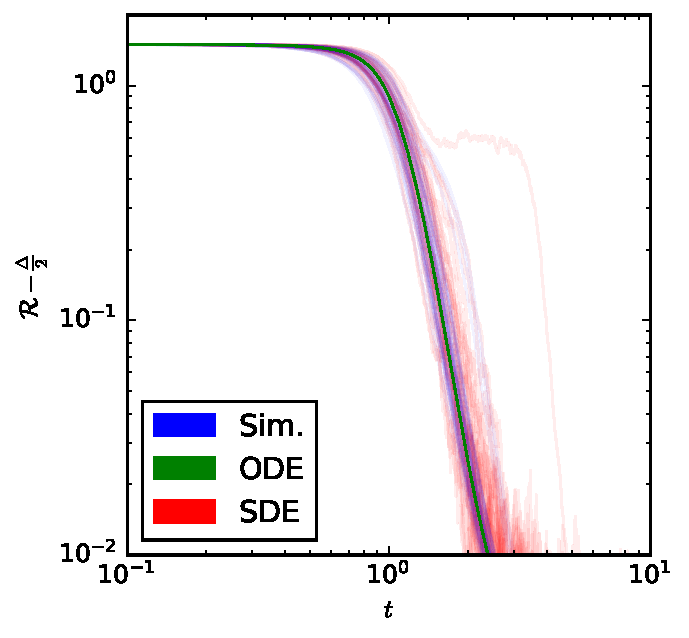
\includegraphics[width=0.44\textwidth]{figs/sde_example_p2}
    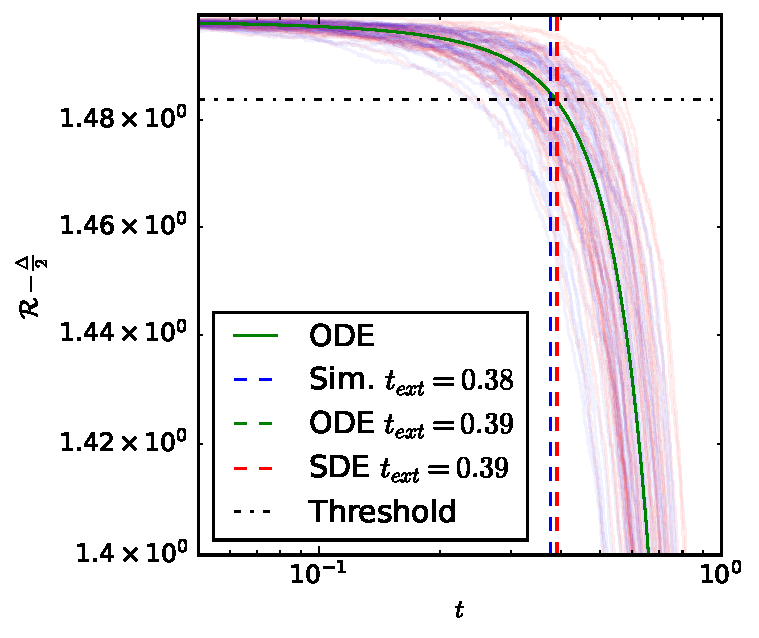
\includegraphics[width=0.49\textwidth]{figs/sde_example_p2-zoom}
    \caption{multiple run of the simulated SGD and the numerically integrated SDE, always starting from the same initial condition, with \(d=3000\).
    All the \(t_\text{ext}\) presented are obtained by solving numerically \eqref{2305:eq:exit_time_implicit_equation}.
    The SDE captures the variance that the ODE doesn't exhibit, but the $t_\text{ext}$ do not change considerably.}
    \label{2305:fig:sde_p2}
\end{figure}

% %%%%%%%%%%%%%%%%%%%%%%%%%%%%%%%%%%%%%%%%%%%%%%%%%%%%%%%%%%%%%%%%%%%%%%%%%%%%%%%
